\documentclass{../doc}

\begin{document}
  \header{Presentation Notes -- Week 2}{
    Private Reading: Quantum Computing \\
    \today \\
    Oberlin College \\
    Iago B. Mendes
  }

  \section{Computational process}
    \begin{itemize}
      \item Registers: Qbits used as input or output
        \begin{equation}
          \ket{x}_n \ket{y}_m
        \end{equation}
        (for $n$ input Qbits and $m$ output Qbits)
      \item Definition of unitary actions:
        \begin{equation}
          \hat U_f (\ket{x}_n \ket{y}_m) = \ket{x}_n \ket{y \oplus f(x)}_m
        \end{equation}
        ``$\oplus$'' = exclusive or (module-2 bitwise addition with no carrying) \\
        Example: $1101 \oplus 0111 = 1010$ \\
        Note:
        \begin{align}
          \hat U_f (\ket{x}_n \ket{0}_m) &= (\ket{x}_n \ket{f(x)}_m) \\
          \hat U_f (\ket{x}_n \ket{1}_m) &= (\ket{x}_n \ket{\tilde f(x)}_m)
        \end{align}
      \item Hadamard transformation:
        \begin{align}
          (\hat H \otimes \hat H) (\ket{0} \otimes \ket{0})
          &= (\hat H \ket{0}) (\hat H \ket{0}) \\
          &= \frac{1}{\sqrt{2}} (\ket{0} + \ket{1}) \frac{1}{\sqrt{2}} (\ket{0} + \ket{1}) \\
          &= \frac{1}{2} (\ket{0}\ket{0} + \ket{0}\ket{1} + \ket{1}\ket{0} + \ket{1}\ket{1}) \\
          &= \frac{1}{2} (\ket{0}_2 + \ket{1}_2 + \ket{2}_2 + \ket{3}_2)
        \end{align}
        For $n$ Qbits:
        \begin{align}
          \hat H^{\otimes n} \ket{0}_n
          &= (\hat H \otimes \hat H \otimes \dots \otimes \hat H) \ket{0}_n \\
          &= \frac{1}{2^{n/2}} \sum_{x=0}^{2^n-1} \ket{x}_n
        \end{align}
      \item ``Quantum parallelism'':
        \begin{align}
          \hat U_f (\hat H^{\otimes n} \otimes \hat 1_m)(\ket{0}_n \ket{0}_m)
          &= \frac{1}{2^{n/2}} \sum_{x=0}^{2^n-1} \hat U_f(\ket{x}_n \ket{0}_m) \\
          &= \frac{1}{2^{n/2}} \sum_{x=0}^{2^n-1} \ket{x}_n \ket{f(x)}_m
        \end{align}
        Note: state depends on all $2^n$ evaluations of $f$ \\
        Wrong typical conclusion: ``Where were all those calculations done? In parallel universes!'' \\
        This is the same mistake as saying that a superposed state is defined, but we don't know what it is. \\\\
        State after measurement: $\ket{x_0} f(x_0)$ \\
        (we only have the evaluation of $f(x_0)$)
    \end{itemize}

  \section{Deutsch's problem}
    \begin{itemize}
      \item Let $f:\{0,1\} \to \{0,1\}$
      \item 4 possibilities:
        \begin{equation*}
          \begin{matrix}
            f(0) & f(1) \\
            0 & 0 \\
            0 & 1 \\
            1 & 0 \\
            1 & 1 \\
          \end{matrix}
        \end{equation*}
      \item Question: is $f$ constant?
      \item Classical computer: 2 evaluations
        \begin{itemize}
          \item Find and compare the values of $f(0)$ and $f(1)$
        \end{itemize}
      \item Quantum computer: 1 evaluation
        \begin{itemize}
          \item Start with $\ket{0}\ket{0}$
          \item Apply $(\hat X \otimes \hat X)$
            \begin{equation}
              \ket{1}\ket{1}
            \end{equation}
          \item Apply $(\hat H \otimes \hat H)$
            \begin{gather}
              \frac12 (\ket{0} - \ket{1}) (\ket{0} - \ket{1}) \\
              \frac12 (\ket{0}\ket{0} - \ket{0}\ket{1} - \ket{1}\ket{0} + \ket{1}\ket{1})
            \end{gather}
          \item Apply $\hat U_f$
            \begin{equation}
              \frac12 (\ket{0}\ket{f(0)} - \ket{0}\ket{\tilde f(0)} - \ket{1}\ket{f(1)} + \ket{1}\ket{\tilde f(1)})
            \end{equation}
            \begin{itemize}
              \item If $f = \text{const}$, $f(1) = f(0)$ and $\tilde f(1) = \tilde f(0)$
                \begin{gather}
                  \frac12 (\ket{0}\ket{f(0)} - \ket{0}\ket{\tilde f(0)} - \ket{1}\ket{f(0)} + \ket{1}\ket{\tilde f(0)}) \\
                  \frac12 (\ket0 - \ket1) (\ket{f(0)} - \ket{\tilde f(0)})
                \end{gather}
              \item If $f \neq \text{const}$, $f(1) = \tilde f(0)$ and $\tilde f(1) = f(0)$
                \begin{gather}
                  \frac12 (\ket{0}\ket{f(0)} - \ket{0}\ket{\tilde f(0)} - \ket{1}\ket{\tilde f(0)} + \ket{1}\ket{f(0)}) \\
                  \frac12 (\ket0 + \ket1) (\ket{f(0)} - \ket{\tilde f(0)})
                \end{gather}
            \end{itemize}
          \item Apply $(\hat H \otimes \hat 1)$ \\
            Note: Hadamard only on the input register
            \begin{itemize}
              \item $f = \text{const}$:
                \begin{gather}
                  \frac12 \frac{1}{\sqrt2} (\ket0 + \ket1 - \ket0 + \ket1) (\ket{f(0)} - \ket{\tilde f(0)}) \\
                  \frac{1}{\sqrt2} \ket1 (\ket{f(0)} - \ket{\tilde f(0)})
                \end{gather}
              \item $f \neq \text{const}$:
                \begin{gather}
                  \frac12 \frac{1}{\sqrt2} (\ket0 + \ket1 + \ket0 - \ket1) (\ket{f(0)} - \ket{\tilde f(0)}) \\
                  \frac{1}{\sqrt2} \ket0 (\ket{f(0)} - \ket{\tilde f(0)})
                \end{gather}
            \end{itemize}
        \end{itemize}
        Answer to problem: $f=\text{const}$ if and only if the input register is 1! \\
        Note: the output register has no use because it can be $f(0)$ or $\tilde f(0)$
      \item Trade-off: in the quantum computation above, we don't find the actual value of the function. That is, we don't know $f(0)$ or $f(1)$. Therefore, we have only eliminated 2 options out of the 4 possibilities for $f$.
    \end{itemize}
  
  \section{Bernstein-Vazirani problem}
    \begin{itemize}
      \item Let $0 \leq a,x < 2^n$ and $f(x) = a \cdot x = a_0 x_0 \oplus a_1 x_1 \oplus \dots$
      \item Question: what is $a$?
      \item Classical computer: $n$ evaluations of $f$
        \begin{itemize}
          \item Find each bit of $a$ with $a \cdot 2^m$ for $0 \leq m < n$ \\
            Note: only the $m$th bit in $2^m$ is 1, all the others are 0
        \end{itemize}
      \item Quantum computer: 1 evaluation
        \begin{itemize}
          \item We can use the same process as before, but the circuit explanation below is more intuitive.
          \item Represent an implementation of $\hat U_f$
            \begin{figure}[H]
              \centering
              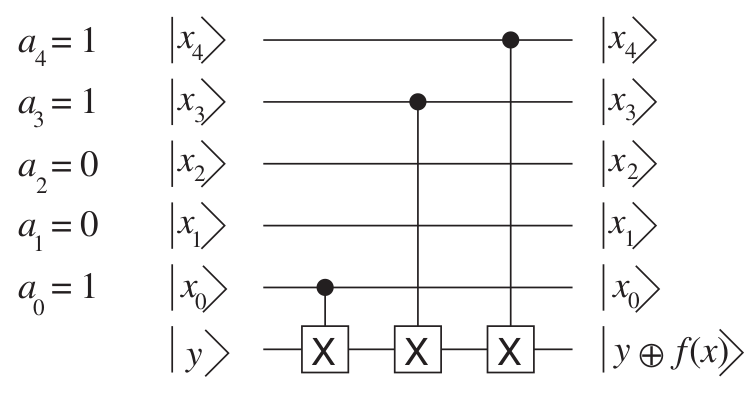
\includegraphics[width=0.4\textwidth]{assets/fig2.8.png}
              \caption{}
            \end{figure}
            In the example above, $a = 11001 = 25$
          \item Sandwich the $\hat U_f$ gate with Hadamard gates
            \begin{figure}[H]
              \centering
              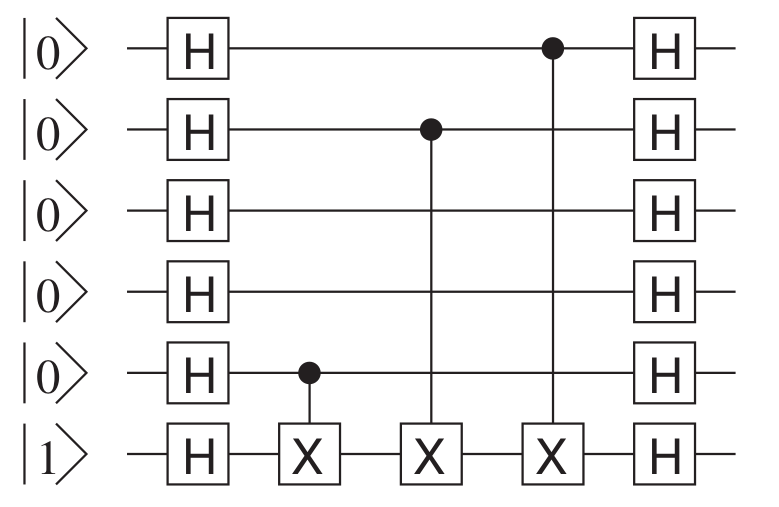
\includegraphics[width=0.3\textwidth]{assets/fig2.9.png}
              \caption{}
            \end{figure}
          \item Use the identity $(\hat H_i \hat H_j) \hat C_{ij} (\hat H_i \hat H_j) = \hat C_{ji}$
            \begin{figure}[H]
              \centering
              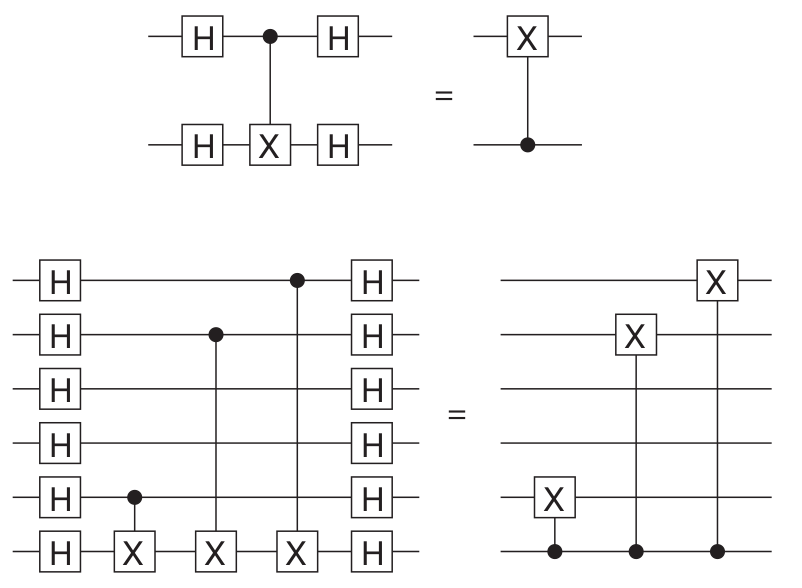
\includegraphics[width=0.4\textwidth]{assets/fig2.10.png}
              \caption{}
            \end{figure}
          \item Now that the output register is the control bit for all cNOT gates, we can create a copy of $a$ in the input registers by setting the output bit to 1
        \end{itemize}
        Mathematically:
        \begin{equation}
          \hat H^{\otimes (n+1)} \hat U_f \hat H^{\otimes (n+1)} \ket0_n \ket1_1 = \ket{a}_n \ket1_1
        \end{equation}
      \item Note: we went from $O(n)$ in the classical computer to $O(1)$ in the quantum computer. \\
        In Simon's problem, we go from $O(2^{n/2})$ to $O(n)$.
    \end{itemize}

\end{document}
